% Copyright (C) 2014-2016 by Thomas Auzinger <thomas@auzinger.name>

\documentclass[draft,final]{vutinfth} % Remove option 'final' to obtain debug information.

\usepackage{listings}
% Load packages to allow in- and output of non-ASCII characters.
\usepackage{lmodern}        % Use an extension of the original Computer Modern font to minimize the use of bitmapped letters.
\usepackage[T1]{fontenc}    % Determines font encoding of the output. Font packages have to be included before this line.
\usepackage[utf8]{inputenc} % Determines encoding of the input. All input files have to use UTF8 encoding.

% Extended LaTeX functionality is enables by including packages with \usepackage{...}.
\usepackage{float}
\usepackage{fixltx2e}   % Provides fixes for several errors in LaTeX2e.
\usepackage{amsmath}    % Extended typesetting of mathematical expression.
\usepackage{amssymb}    % Provides a multitude of mathematical symbols.
\usepackage{mathtools}  % Further extensions of mathematical typesetting.
\usepackage{microtype}  % Small-scale typographic enhancements.
\usepackage{enumitem}   % User control over the layout of lists (itemize, enumerate, description).
\usepackage{multirow}   % Allows table elements to span several rows.
\usepackage{booktabs}   % Improves the typesettings of tables.
\usepackage{subcaption} % Allows the use of subfigures and enables their referencing.
\usepackage[ruled,linesnumbered,algochapter]{algorithm2e} % Enables the writing of pseudo code.
\usepackage[usenames,dvipsnames,table]{xcolor} % Allows the definition and use of colors. This package has to be included before tikz.
\usepackage{nag}       % Issues warnings when best practices in writing LaTeX documents are violated.
\usepackage{hyperref}  % Enables cross linking in the electronic document version. This package has to be included second to last.
\usepackage[acronym,toc]{glossaries} % Enables the generation of glossaries and lists fo acronyms. This package has to be included last.

% Define convenience functions to use the author name and the thesis title in the PDF document properties.
\newcommand{\authorname}{Kevin Haller} % The author name without titles.
\newcommand{\thesistitle}{Title} % The title of the thesis. The English version should be used, if it exists.

% Set PDF document properties
\hypersetup{
    pdfpagelayout   = TwoPageRight,           % How the document is shown in PDF viewers (optional).
    linkbordercolor = {Melon},                % The color of the borders of boxes around crosslinks (optional).
    pdfauthor       = {\authorname},          % The author's name in the document properties (optional).
    pdftitle        = {\thesistitle},         % The document's title in the document properties (optional).
    pdfsubject      = {Subject},              % The document's subject in the document properties (optional).
    pdfkeywords     = {a, list, of, keywords} % The document's keywords in the document properties (optional).
}

\setsecnumdepth{subsection} % Enumerate subsections.

\nonzeroparskip             % Create space between paragraphs (optional).
\setlength{\parindent}{0pt} % Remove paragraph identation (optional).


\newacronym{lod}{LOD}{Linked Open Data}

\makeindex      % Use an optional index.
\makeglossaries % Use an optional glossary.
%\glstocfalse   % Remove the glossaries from the table of contents.

% Set persons with 4 arguments:
%  {title before name}{name}{title after name}{gender}
%  where both titles are optional (i.e. can be given as empty brackets {}).
\setauthor{}{\authorname}{}{male}
\setadvisor{Pretitle}{Reka Marta Sabou}{Posttitle}{female}

% For bachelor and master theses:
\setfirstassistant{Pretitle}{Forename Surname}{Posttitle}{male}
\setsecondassistant{Pretitle}{Forename Surname}{Posttitle}{male}
\setthirdassistant{Pretitle}{Forename Surname}{Posttitle}{male}

% For dissertations:
%\setfirstreviewer{Pretitle}{Forename Surname}{Posttitle}{male}
%\setsecondreviewer{Pretitle}{Forename Surname}{Posttitle}{male}

% For dissertations at the PhD School:
%\setsecondadvisor{Pretitle}{Forename Surname}{Posttitle}{male}

% Required data.
\setaddress{Address}
\setregnumber{1325694}
\setdate{01}{08}{2016} % Set date with 3 arguments: {day}{month}{year}.
\settitle{\thesistitle}{Titel der Arbeit} % Sets English and German version of the title (both can be English or German).
\setsubtitle{Optional Subtitle of the Thesis}{Optionaler Untertitel der Arbeit} % Sets English and German version of the subtitle (both can be English or German).

% Select the thesis type: bachelor / master / doctor / phd-school.
% Bachelor:
\setthesis{bachelor}
%
% Master:
%\setthesis{master}
%\setmasterdegree{dipl.} % dipl. / rer.nat. / rer.soc.oec. / master
%
% Doctor:
%\setthesis{doctor}
%\setdoctordegree{rer.soc.oec.}% rer.nat. / techn. / rer.soc.oec.
%
% Doctor at the PhD School
%\setthesis{phd-school} % Deactivate non-English title pages (see below)

% For bachelor and master:
\setcurriculum{Software and Information Engineering}{Software und Information Engineering} % Sets the English and German name of the curriculum.

% For dissertations at the PhD School:
\setfirstreviewerdata{Affiliation, Country}
\setsecondreviewerdata{Affiliation, Country}

% Define convenience macros.
\newcommand{\todo}[1]{{\color{red}\textbf{TODO: {#1}}}} % Comment for the final version, to raise errors.

\begin{document}

% Acronyms
\newacronym{geo}{GEO}{Basic Geo (WGS84 long/lat) Vocabulary}
\newacronym{lov}{LOV}{Linked Open Vocabulary}

\frontmatter % Switches to roman numbering.
% The structure of the thesis has to conform to
%  http://www.informatik.tuwien.ac.at/dekanat

\addtitlepage{naustrian} % German title page (not for dissertations at the PhD School).
\addtitlepage{english} % English title page.
\addstatementpage

\begin{danksagung*}
\todo{Ihr Text hier.}
\end{danksagung*}

\begin{acknowledgements*}
\todo{Enter your text here.}
\end{acknowledgements*}

\begin{kurzfassung}
\todo{Ihr Text hier.}
\end{kurzfassung}

\begin{abstract}
\todo{Enter your text here.}
\end{abstract}

% Select the language of the thesis, e.g., english or naustrian.
\selectlanguage{english}

% Add a table of contents (toc).
\tableofcontents % Starred version, i.e., \tableofcontents*, removes the self-entry.

% Switch to arabic numbering and start the enumeration of chapters in the table of content.
\mainmatter

\chapter{Introduction}

\section{Motivation}
\todo{Intro Web of Documents, missed potential, isolated data sources}

The same applies at the moment to the Vienna University of Technology. In order to find a special location like a certain lecture hall and how it can be accessed without obstacles like stairways, one has to search for information on web sites, scan floor plans and eventually construct a convenient route to the location based on the gathered knowledge. For humans this procedure does not constitute a problem, but think of machines.
\todo{Elaborate on problem for machines, Deep learning, NLP state of the art reference}
 %Web sites are usually designed to present information in a human-readable way and as for images there is in general at the moment of writing no sophisticated approach to interpret such content by machines without additional support of humans. 

As a consequence the barrier for application developers is quite high due to the time consuming task of gathering and extracting the data from multiple sources and transforming it into a representation that is usable by the planned application.

\todo{Linked Data, goal of thesis}

\section{Problem description}
\label{intro-problem-description}

\todo{more comprehensive description}

\begin{itemize}
	\item prototype of a map application based on the transformation of spatial data of the Vienna University of Technology into Linked Data to evaluate and discuss the potential benefits and caveats. 
	\item prototype of an ontology to model spatial data as well as the indoor plans of facilities taking accessibility into consideration. In compliance to best practises terms of already existing ontologies shall be reused whenever possible.
	\item linking of the transformed spatial data with external sources like GeoNames or LinkedGeoData. 
\end{itemize}

\section{Structure of the thesis}
This chapter outlined the motivation for writing this thesis and gave a description of the problems for which a solution will be suggested. The rest of this thesis is structured as follows: Chapter \ref{background-chapter} discusses the basic concepts, principles and technologies that build the foundation of Linked Data and the Semantic Web. It is intended to be a brief introduction for readers that are not familiar with this topic. Chapter \ref{related-work-chapter} provides a summary of past efforts in research and works related to the focus of this thesis. In the subsequent chapter \ref{solution-chapter} a solution for the given problems will be suggested and discussed. This includes the prototype of an ontology that models the problem domain as well as an architectural prototype of a system that manages a subset of spatial data about the Vienna University of Technology in form of Linked Data and provides a human- and machine-friendly interface to it. Finally, the implemented solution is evaluated and conclusions are drawn in the last chapter \ref{discussion-chapter}. It provides furthermore an outlook to future work and potential improvements. 


\chapter{Background}
\label{background-chapter}

\section{Semantic Web}
\todo{Enter your text here.}

\section{RDF}
\todo{Enter your text here.}

\section{Ontology}
\todo{Enter your text here.}

\subsection{RDFS}
\todo{Enter your text here.}

\subsection{OWL}
\todo{Enter your text here.}

\section{SPARQL}
\todo{Enter your text here.}

\chapter{Related Work}
\label{related-work-chapter}

In this chapter important efforts and research related to this thesis are outlined. Section \ref{related-work-geospatial-ontologies} describes and evaluates geospatial ontologies that were suggested by \cite{tandy_spatial_????} or discovered in the dataset of \gls{lov} through a systematic search.  

\section{Geospatial ontologies}
\label{related-work-geospatial-ontologies}
This section is going to outline common ontologies for describing geospatial data and to evaluate them from the perspective of the given problem description (see \ref{intro-problem-description}).The ontologies were either be suggested by \cite{tandy_spatial_????} or discovered in the dataset of \gls{lov} by common spatial search terms like \textit{'feature'}, \texit{'geometry'} or \textit{'location'}. \textit{Feature} and \textit{Geometry} are widely used terms in these ontologies and describe two different concepts of geospatial science. A \textit{feature}  is simply a spatial entity that can be everything from a building with fixed position to a movable food truck as long as it has a spatial extent. \textit{Geometry} as the name suggests is a certain geometric shape from points, lines to polygons. Geometric shapes can be used to describe  the spatial extent of \textit{features}.

\subsection{Basic Geo Vocabulary (WGS84)}
\label{related-work-geospatial-ontologies-wgs84}

\gls{geo}\cite{brickley_basic_2003} is a lightweight ontology published by W3C to describe the position of a spatial \textit{feature} using the WGS84 geodetic reference datum\footnote{\url{http://en.wikipedia.org/wiki/World_Geodetic_System}} with the properties \texttt{longitude}, \texttt{latitude} and \texttt{attitude}. The general class \texttt{SpatialThing} is the domain of all these properties. Figure \ref{fig:related-work-geospatial-ontologies:wgs84} shows a visualization of this ontology.

\begin{figure}[H]
    \centering
    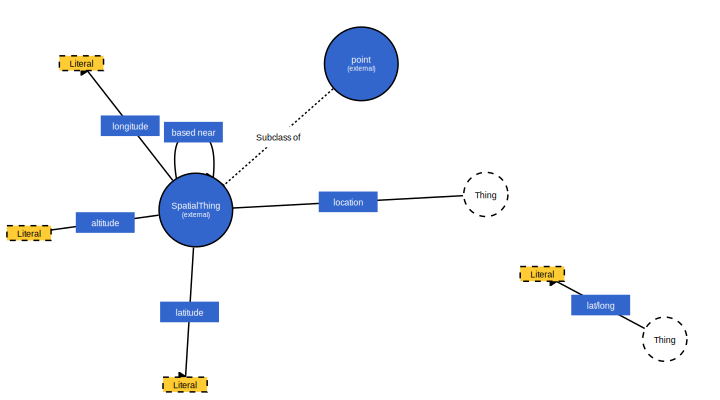
\includegraphics[width=0.75\textwidth]{graphics/vocabularies/wgs84.png}
    \caption{Visualization of Basic Geo Vocabulary}
    \label{fig:related-work-geospatial-ontologies:wgs84}
\end{figure}

Advantages are it`s simplicity and popularity as an analysis of the LOD cloud\cite{research_group:_akws_lodstats_????} indicates. This analysis shows that \gls{geo} is used in \textbf{538} different datasets in the LOD cloud and is thereby the 4th most used ontology regarding usage in different datasets. It is used by big players like DBpedia\footnote{\url{http://dbpedia.org}}, LinkedGeoData\footnote{\url{http://linkedgeodata.org/About}} and GeoNames\footnote{\url{http://linkedgeodata.org/About}}. 
Listing \ref{lst:related-work-geospatial-ontologies:wgs84-dbpedia} shows a data snippet of DBpedia describing the town square 'Karlsplatz' in Vienna with \gls{geo}.

\begin{lstlisting}[frame=single, caption=Snippet of DBpedia, label={lst:related-work-geospatial-ontologies:wgs84-dbpedia}]
@prefix dbr:  <http://dbpedia.org/resource/> .
@prefix geo:  <http://www.w3.org/2003/01/geo/wgs84_pos#> .

dbr:Karlsplatz  rdf:type  geo:SpatialThing ;
  rdfs:label  "Karlsplatz"@en , "Karlsplatz (Wien)"@de ;
  geo:lat     "48.19916534423828125"^^xsd:float ;
  geo:long    "16.370000839233398438"^^xsd:float .
\end{lstlisting}

\gls{geo} evolved into a standard for presenting the location of points of interest and  as pointed out by best practices \cite{hyland_best_2014}, the use of standardized ontologies to describe one`s data facilitates inclusion into the Web of Data. 

However, this ontology is not sufficient for describing spatial data more complex than a single point in a coordinate reference system.


\subsection{schema.org}
...

\subsection{NeoGeo Geometry Ontology}
...

\subsection{GeoSPARQL}
...

\subsection{ISA Programme Location Core Vocabulary}
...


\section{Linked Open Data based map applications}
\label{related-work-map-app}


\todo{Existing map application based on Linked Open Data, Southampton, Oxford, LODUM}


\section{Accessibility ontologies}
\label{related-work-accessibility-ontologies}
\todo{Evaluation of accessibility ontologies as related work for the designed ontology prototype}

\section{Indoor modelling}
\label{related-work-accessibility-ontologies}
\todo{Indoor modelling research}

\chapter{Solution}
\label{solution-chapter}

\section{Data sources}
\todo{A description of the data sources and the transformation process}

\section{Prototype of ontology}
\todo{Description of the developed ontology with newly created terms and reused ones, and why using GeoSPARQL and what are the disadvantages}

\section{Architectural prototype}
\todo{A description of the system, the different layers, integration, linking and web framework, REST API, used technologies}

\subsection{System architecture}
\todo{Description of the system architecture}

\subsection{RDF Framework}
\todo{Reasoning why using Sesame, not Apache Jena}

\subsection{Linked Data management}
\todo{Description of the data management and compliance to best practise}

\subsection{Linking}
\todo{Description of strategies for linking with external sources and to enrich the data}

\subsection{Linked Data publishing}
\todo{Description of the data publishing and compliance to best practise}

\section{Web application}
\todo{A more comprehensive presentation of the user interface for humans to show the targeted use case.}

\chapter{Discussion}
\label{discussion-chapter}

\section{Evaluation}
\todo{Enter your text here.}

\section{Further work}
\todo{Enter your text here.}

\section{Conclusion}

\todo{Enter your text here.}

% Remove following line for the final thesis.
\input{intro.tex} % A short introduction to LaTeX.

\backmatter

% Use an optional list of figures.
\listoffigures % Starred version, i.e., \listoffigures*, removes the toc entry.

% Use an optional list of tables.
\listoftables % Starred version, i.e., \listoftables*, removes the toc entry.

% Use an optional list of alogrithms.
\listofalgorithms
\addcontentsline{toc}{chapter}{List of Algorithms}

% Add an index.
\printindex

% Add a glossary.
\printglossaries

% Add a bibliography.
\bibliographystyle{plain}
\bibliography{thesis}

\end{document}